\documentclass[11pt,a4paper,oneside]{article}
\usepackage[dvipsnames, svgnames, x11names]{xcolor}
\usepackage{euler,amssymb,amsthm,amsmath,amsfonts,graphicx,epigraph,indentfirst,enumerate,comment,listings,fontspec,color,subcaption,listings}
\usepackage{xeCJK}
\usepackage{hw}
\usepackage{pythonhighlight}
\usepackage{tikz}
\usepackage{algorithm}
\usepackage{algpseudocode}
\usepackage{float}

\newtheorem{theorem}{Theorem}
\newcommand{\nth}[1]{#1\textsuperscript{th}}
\newcommand{\E}{\mathop{\mathbb{E\/}}}
\newcommand{\R}{\mathbb{R}}
\newcommand{\norm}[1]{\|#1\|}


\renewcommand{\hwtitle} {CS217 Homework 5, First Submission}	
\renewcommand{\hwauthor}{Akina}
\renewcommand{\hwdate}{May 8, 2020}

\begin{document}
\title{\hwtitle}
\author{\hwauthor}
\date{\hwdate}
\maketitle



\setcounter{section}{4}
\section*{Flows with Vertex Capacities}


\begin{problem}{1}
	\statement
    Let $G = (V,c)$ be a flow network. Prove that flow is ``transitive'' in the following sense: if $r,s,t$ are vertices, 
    and there is an $r$--$s$-flow of value $k$ and an $s$--$t$-flow of value $k$, then there is an $r$--$t$-flow of 
    value $k$.
    
    \solution
    There must be a minimum $r-t$-cut in graph $G$, denoted $S_{r-t}$. Then  either $s \in S_{r-t}$ or $s \in V \backslash S_{r-t} $.\\
    If $s \in S_{r-t}$, then $S_{r-t}$ is also a $s - t$-cut. If we denote the minimum $s-t$-cut $S_{s-t}$, then $cap(S_{r-t}) \ge cap(S_{s-t})$. Applying the max-flow-min-cut theorem, $cap(S_{s-t})$ is the maxflow, which is not less than $k$. Accordingly, $cap(S_{r-t}) \ge cap(S_{s-t}) \ge k$.\\
    If $s \in V \backslash S_{r-t}$, then $S_{r-t}$ is also a $r - s$-cut. Similarly, $cap(S_{r-t}) \ge k$.\\
    Hence, $cap(S_{r-t}) \ge k$ in both condition. Then apply the max-flow-min-cut theorem again, the maximum $r - t$-flow value $maxflow = mincut = cap(S_{r - t}) \ge k$.\\
    Therefore there exists an $r-t$-flow of value $k$;
\end{problem}

\section*{Vertex Disjoint Paths}

Let $G$ be a directed graph. Two paths $p_1, p_2$ from $s$ to $t$ are called {\em vertex disjoint}
if they don't share any vertices except $s$ and $t$. 

\begin{theorem}[Menger's Theorem]
   Let $G$ be a graph and $s \ne t$ two vertices therein. Let $k \in \mathbf{N}_0$. 
   Then exactly one of the following is true:
   \begin{enumerate}
   \item There are $k$ vertex disjoint paths $p_1,\dots,p_k$ from $s$ to $t$; that is, no two $p_i$, $p_j$ share
   any vertex besides $s$ and $t$.
   \item There are vertices $v_1,\dots,v_{k-1} \in V \setminus \{s,t\}$ such that
   $G - \{v_1,\dots, v_{k-1}\}$ contains no $s$--$t$-path.
   \end{enumerate}
\end{theorem}

\begin{problem}{3}
	\statement
   Prove Menger's Theorem. You have to prove two things: first, not both cases above can occur (this is rather easy);
   second, one of them must occur (this requires a tool from the lecture).
   
    \solution
    First, prove not both cases above can occur.\\
    For any graph $G$ with $k$ vertex disjoint paths, any $v \in V \backslash \{ s,t \}$ can occur in at most 1 path $p$, for no two $p_i,p_j$ share any vertex besides $s$ and $t$. So the rest of $k - 1$ paths remains existent. By removing a $v \in V \backslash \{ s,t \}$, the number of disjoint paths at most decrease by 1. So $G - {v_1,\dots,v_{k - 1}}$ contains at least 1 $s-t$-path. So case 2 doesn't occur.\\
    Second, prove one of them must occur.\\
    We can create a new directed graph $G'$.\\
    Consider all the $v_i \in V \backslash \{ s,t \}$, for any edge $(u,v_i)$ in $G$, there's an edge $(u,{v_{in}}_i)$ in $G'$. And for any edge $(v_i,u)$ in $G$, there's an edge $({v_{out}}_i,u)$ in $G'$. All the edges above has an infinite capacity.\\
    There are also 1-capacity edges $({v_{in}}_i,{v_{out}}_i) ,\forall i$ in $G'$.\\
    It is obvious that the maximum flow of $G'$ is the number of disjoint $s-t$-path in $G$, for any flow on $s-t$ path is limited by 1 and any of two joint paths share at least one 1-capacity edge.\\
    If case 1 doesn't occur, then there's at most $k - 1$ vertex disjoint $s-t$-paths, means the maximum flow of $G'$ is at most $k - 1$. So the minimum cut of $G'$ is also less than $k - 1$. Therefore, there exists a minimum cut $S$ such that $\exists v_1,\dots,v_{k-1} \in V \backslash \{ s,t \}$, ${v_{in}}_1,\dots,{v_{in}}_{k-1} \in S$, while ${v_{out}}_1,\dots,{v_{out}}_{k-1} \notin S$. So in $G-{v_1,\dots, v_{k - 1}}$ there's no $s-t$-path, case 2 occuring.\\
    Accordingly, Menger's theorem holds.

\end{problem}



Let $V = \{0,1\}^n$. The $n$-dimensional Hamming cube $H_n$ is the graph $(V,E)$ where
$\{u,v\} \in E$ if $u,v$ differ in exactly one coordinate.
Define the $\nth{i}$ level of $H_n$ as 
\begin{align*}
  L_i := \{u \in V \ | \ \norm{u}_1 = i \} \ ,
\end{align*}
i.e., those vertices $u$ having exactly $i$ coordinates which are $1$.
\begin{center}
  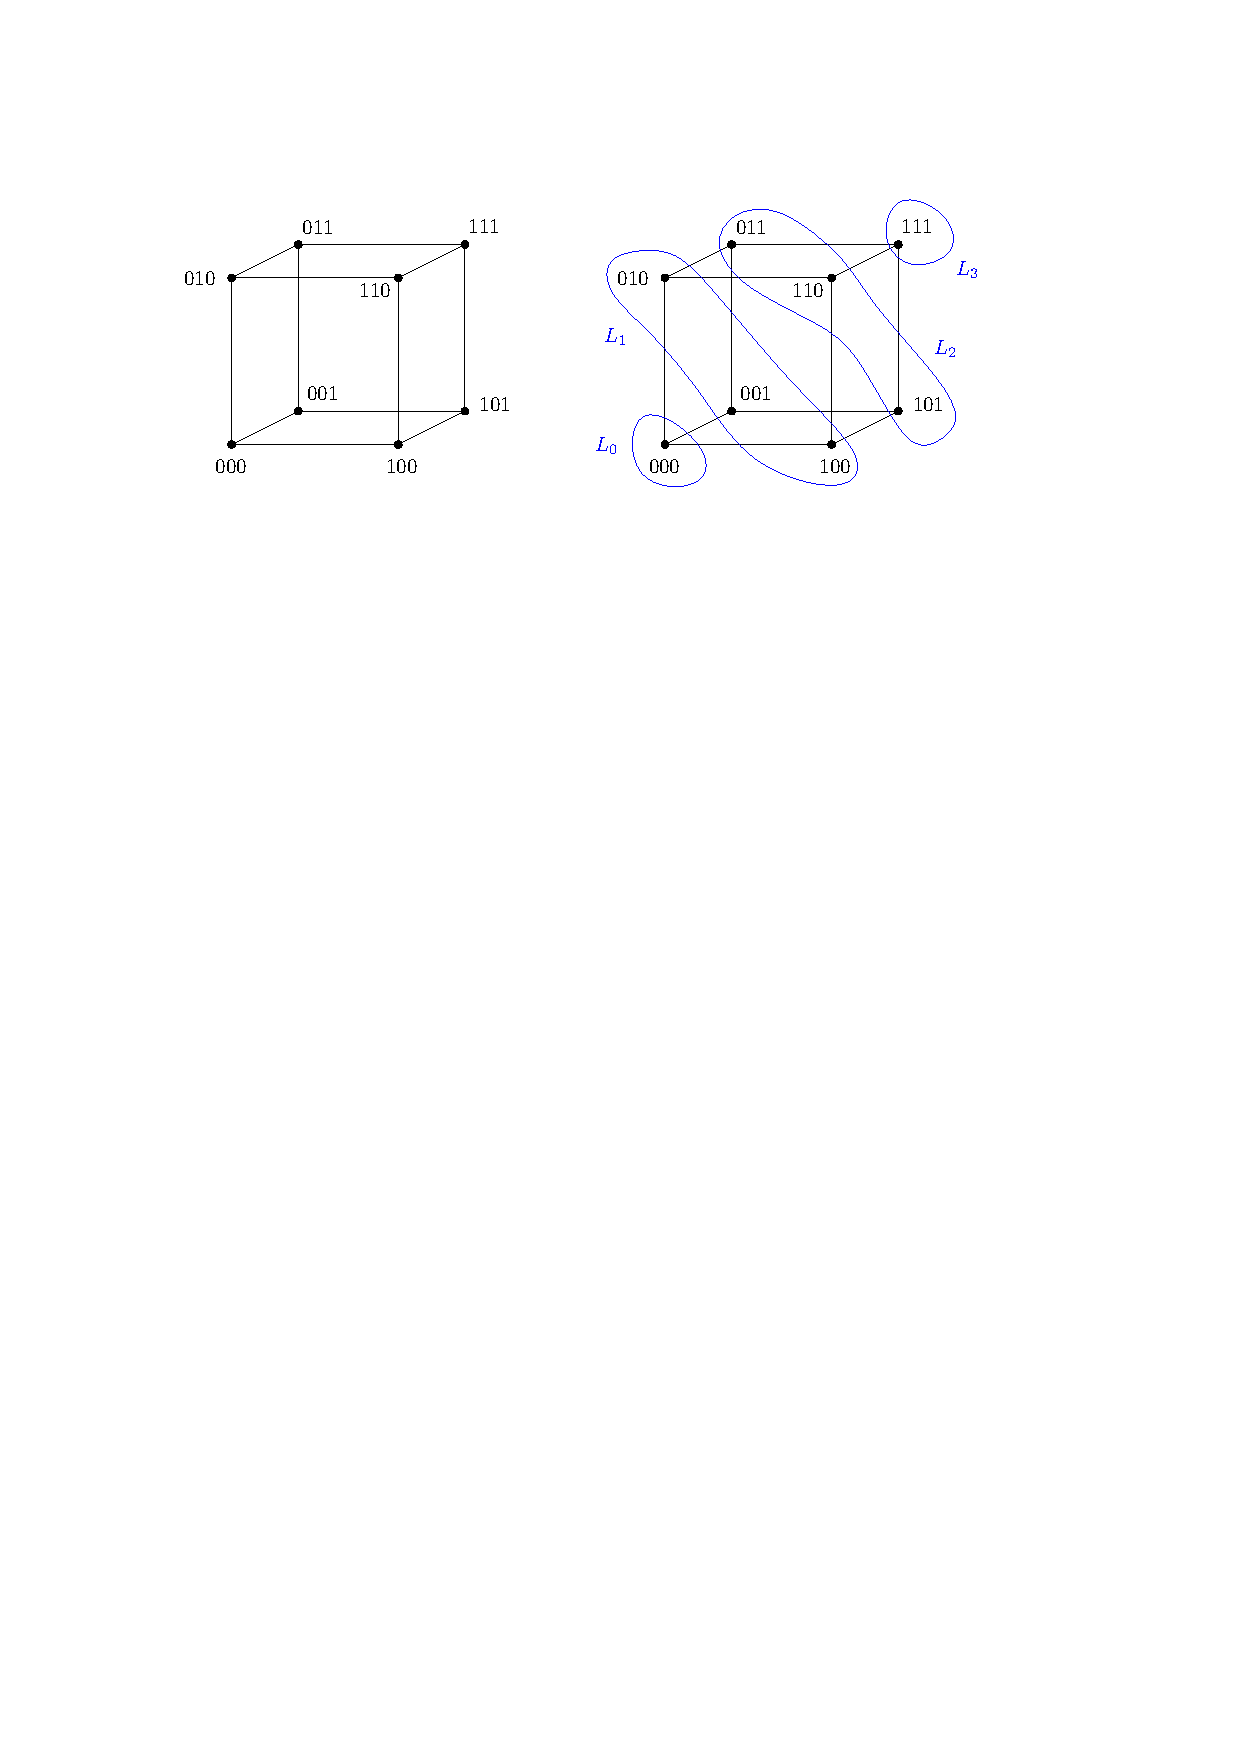
\includegraphics[width=0.8\textwidth]{figures/hamming-3-dim.pdf}\\
  {\small The $3$-dimensional Hamming cube and the four 
    sets $L_0$, $L_1$, $L_2$, $L_3$.}
\end{center}


\begin{problem}{4}
  \statement
  Consider the induced bipartite subgraph $H_n[ L_i \cup L_{i+1}]$. This is 
  the graph on vertex set $L_i \cup L_{i+1}$ where two edges are connected
  by an edge if and only if they are connected in $H_n$.
  Show that for $i < n/2$ the graph $H_n[ L_i \cup L_{i+1}]$
  has a matching of size $|L_i| = {n \choose i}$.
  
  \solution
  \begin{proof}
    $|L_i| = {n \choose i}$, $|L_{i + 1}| =  {n \choose {i + 1}}$. Consider build a flow network from $s$ to $t$ that:
    \begin{enumerate}
      \item $s$ connected to all nodes in $L_i$ with capacity $1$
      \item all nodes in $L_{i + 1}$ connected to $t$ with capacity $1$
      \item preserve all edges in the bipartite graph formed by $L_{i}, L_{i + 1}$, assign them with capacity $1$ and direction from $L_{i}$ to $L_{i + 1}$
    \end{enumerate}
    The maximum flow is at most $|L_{i}|$, since there's a cut $\{s\}$ that the sum of capacity of edges across the cut is $L_{i}$. We are to prove that maximum flow is at least $|L_{i}|$. 

    Nodes in $L_{i}$ has $u := n - i$ out degree each -- they have $i$ ones and $n - i$ zeros, and connected to those who change a zero to one. Similarly, nodes in $L_{i + 1}$ has $v := i + 1$ in degree each. Since $i < n / 2$, $u \geq v$. Now we assign flows in edges:
    \begin{enumerate}
      \item $s$ connected to all nodes in $L_i$ : $1$
      \item all nodes in $L_{i + 1}$ connected to $t$ : $\frac {{n \choose i}} {{n \choose {i + 1}}} = \frac {i + 1} {n - i} = \frac v u$
      \item all edges in the bipartite graph formed by $L_{i}, L_{i + 1}$ : $\frac 1 u$
    \end{enumerate}
 
    It's obvious that such assignment satisfies all flow condition and has a value of $|L_i|$. So maximum flow is at least $L_i$. With previous arguments, the maximum flow \textit{equals to} $|L_i|$.
 
    Node that the capacity of edges are all integers, we can always obtain a integral flow by algorithm like dinic. Pick all the edges from $L_{i}$ to $L_{i + 1}$ with flow passes by, it's a matching with size $|L_i|$.
    
  \end{proof}
\end{problem}


\begin{problem}{5}
	\statement
  Let $H_n$ be the $n$-dimensional Hamming cube. For $i < n/2$ consider
  $L_i$ and $L_{n-i}$. Note that 
  $|L_i| = {n \choose i} = { n \choose n-i}  = L_{n-i}$, so the 
  $L_i$ and $L_{n-i}$ have the same size.   Show that there are ${n \choose i}$ paths $p_1,p_2,\dots,p_{ {n \choose i}}$
  in $H_n$ such that

  (i) each $p_i$ starts in $L_i$ and ends in $L_{n-i}$; \\
  (ii) two different paths $p_i,p_j$ do not share any vertices.
  
    \solution
    \begin{proof}
      It's nearly the same way as task $4$ to solve this problem, and use task $3$'s technique to avoid path intersection.  

      We now construct a flow graph from $s$ to $t$. Pick all nodes and edges between $L_i$ and $L_{n - i}$, assign edges with direction from lower labels to higher. Connect $s$ to all nodes in $L_i$, and all nodes in $L_{n - i}$ to $t$. What's more we split nodes in $L_i \cdots L_{n - i}$ each into two, one takes all in degree and another takes all out degree, and connected an edge from \textit{in} to \textit{out}, calling it \textit{inner edge}. Assign all edges with capacity $1$.

      Now consider construct a flow. All \textit{inner edges} in $L_x$ take flow of $\frac {|L_x|} {|L_i|}$, which is not greater than $1$ obviously. All edge from $L_{x}$ to $L_{x + 1}$ take flow $\frac {|L_x|} {|L_i| \cdot (n - x)}$. All edges from $S$ or to $T$ take flow $1$.
      
      It's a proper flow in the graph, simply observing its symmetricity. Considering that the cut $\{s\}$ is a cut with value $|L_i|$, the maximum flow is $|L_i|$. By dinic there's another integral maximum flow, so by result of task $3$ we can announce two properties hold if we obtain paths by spliting this flow.
    \end{proof}
\end{problem}


\section*{Matchings and Vertex Covers}

The following exercise was on the final exam of CS 499 (mathematical foundations of computer science) in spring 2019.

\begin{problem}{6}
	\statement
    Let $\nu(G)$ denote the size of a maximum matching of $G$. Show that a bipartite graph $G$
    has at most $2^{\nu(G)}$ minimum vertex covers.
    
    \solution
    Select a maximum matching $M$ of $G$. 
    Edges in $M$ don't share any vertex, so a minimum vertex cover should include at least one vertex in each edge of $M$. 
	And because $G$ is a bipartite graph, Konig's Theorem implies that $\nu(G)$ = $\min|C|$. 
    So a minimum vertex cover should include exactly one vertex in each edge of $M$, and doesn't include any other vertex. 
    A minimum vertex cover has at most 2 choices to cover a edge in $M$ and $M$ has $\nu(G)$ edges, 
    so $G$ has at most $2^{\nu(G)}$ minimum vertex covers. 
\end{problem}

Obviously, this is not  true for general (non-bipartite) graphs: the triangle $K_3$ has $\nu(K_3) = 1$ but it has 
three minimum vertex covers. The five-cycle $C_5$ has $\nu(C_5) = 2$ but has five minimum vertex covers.

\begin{problem}{7}
	\statement
   Is there a function $f: \mathbf{N}_0 \rightarrow \mathbf{N}_0$ such that every graph with $\nu(G) = k$ has 
   at most $f(k)$ minimum vertex covers? How small a function $f$ can you obtain?
   
    \solution   
    Select a maximum matching $M$ of $G$ with $|M|=k$. 
    If both vertex of an edge in $G$ aren't included in $M$, then this edge can be added into $M$ to make a larger matching, 
    so every edge of $G$ has at least 1 vertex in $M$.
    
	
	For a minimum vertex cover $C$,define $C\cap M = N$ and $G'=\{ e\in E | e\cup N=\emptyset\}$. 
	Because every edge of $G$ has at least 1 vertex in $M$, all edges in $G'$ has at least 1 vertex in $M/N$, which means the vertex won't appear in $C$. 
	If there is a edge in $G'$ with both vertexes in $M/N$, then this edge isn't covered by $C$. 
	For every edge in $G'$ with one vertex in $M/N$, the other vertex should be included in $C$ to cover this edge, 
	and by adding these vertexes a minimum vertex cover is made.
	Therefore, $C$ can be generated with $N$ in a definite way.

	Because $M$ has k edges and in each edge at least 1 vertex should be included to cover itself, there exists at most $3^k$ ways to select $N$ from $M$.
	Therefore the number of minimum vertex covers is $3^k$ at most.
	$f(k)=3^k$ can be obtained, and it's exactly the number of minimum vertex covers when $G$ is composed of k triangle $K_3$.
\end{problem}


\end{document}